\newpage
\section{Datensammlung bereinigen}

Die Vorarbeit hat eine Datensammlung von etwa 370'000 Nachrichtenartikeln ergeben, die jeweils über eine eindeutige URL verfügen. 
Wir haben durch die Verwendung von Unique Constraints sichergestellt, dass jede URL einzigartig ist. 
Allerdings vermuteten wir, dass die Datensammlung Duplikate von Texten enthält, die unter verschiedenen URLs veröffentlicht wurden. 
Dies könnte durch Weiterleitungen auf andere Seiten oder veränderte URLs verursacht worden sein. 
Um eine genaue Aussage über den Gender Gap in diesen Nachrichtenportalen machen zu können, mussten wir alle Duplikate pro Nachrichtenportal eliminieren. 

Nach einigen Testversuchen mit 1000 Artikeln entschieden wir uns dafür, die \gl{cosine-similarity} zu verwenden, um Artikeltexte untereinander zu vergleichen. 
Dieser Vergleich war bei den Tests performanter als die \gl{levenshtein-similarity}, die ebenfalls zur Auswahl stand. 
Der Rechenaufwand für den Vergleich zweier Zeichenketten der Länge m bzw. n ist bei der \gl{levenshtein-similarity} 
\(O(m*n)\), während er bei der \gl{cosine-similarity} nur \(O(m+n)\) beträgt
\footnote{https://pypi.org/project/strsimpy/}.

Die \gl{cosine-similarity} ist eine Metrik zur Messung der Ähnlichkeit zwischen zwei Vektoren.
Sie definiert die Ähnlichkeit zwischen zwei Vektoren als den Kosinus des Winkels zwischen ihnen.
In unserem Fall sind die Vektoren die Artikeltexte repräsentiert im Vector Space Modell. 
Um die Ähnlichkeit zwischen einem Vektor und einer Menge von anderen Vektoren zu berechnen, erstellen wir eine Ähnlichkeitsmatrix. 
Wenn der Kosinus 1 ist, sind die Texte gleich. 
Als Schwellwert für die Ähnlichkeit haben wir 0.9 festgelegt, da dieser bei unseren Tests am besten funktionierte. 
Wenn wir einen höheren Schwellwert genommen hätten, hätten wir nicht alle Duplikate gefunden und bei einem zu niedrigen Schwellwert
hätten wir zu viele Texte als Duplikate interpretiert, die gar keine sind. 

Da jeder Artikeltext mit jedem anderen verglichen werden muss, hätte der Algorithmus eine Matrix in der Grösse 
von 371'653 x 371'653 erstellen müssen und 42,9 GB Arbeitsspeicher benötigt. 
Das war für unsere Arbeitsmaschinen zu viel. 
Daher haben wir das \enquote{divide and conquer} Verfahren angewendet und aus einem grossen Problem kleine Teilprobleme gemacht. 
Für jeden Artikel, den wir verglichen haben, haben wir eine neue Matrix erstellt, sodass sie nur noch 1x371'653 gross war und dann nacheinander 371'653 Mal verglichen wurde. 
Wir gingen damit einen Tradeoff ein, der die Ausführungszeit verlängerte, die der Algorithmus benötigte. Das erstellte Skript benötigte zwei Tage um alle Duplikate zu finden.

Auf diese weise konnten wir alle Duplikate und nahezu-Duplikate aus der Datenbank entfernen.
Die Abbildung \ref{duplicates} gibt einen Überblick über die entfernten Artikel pro Nachrichtenportal.

\begin{figure}[H]
	\begin{center}
        \centering
		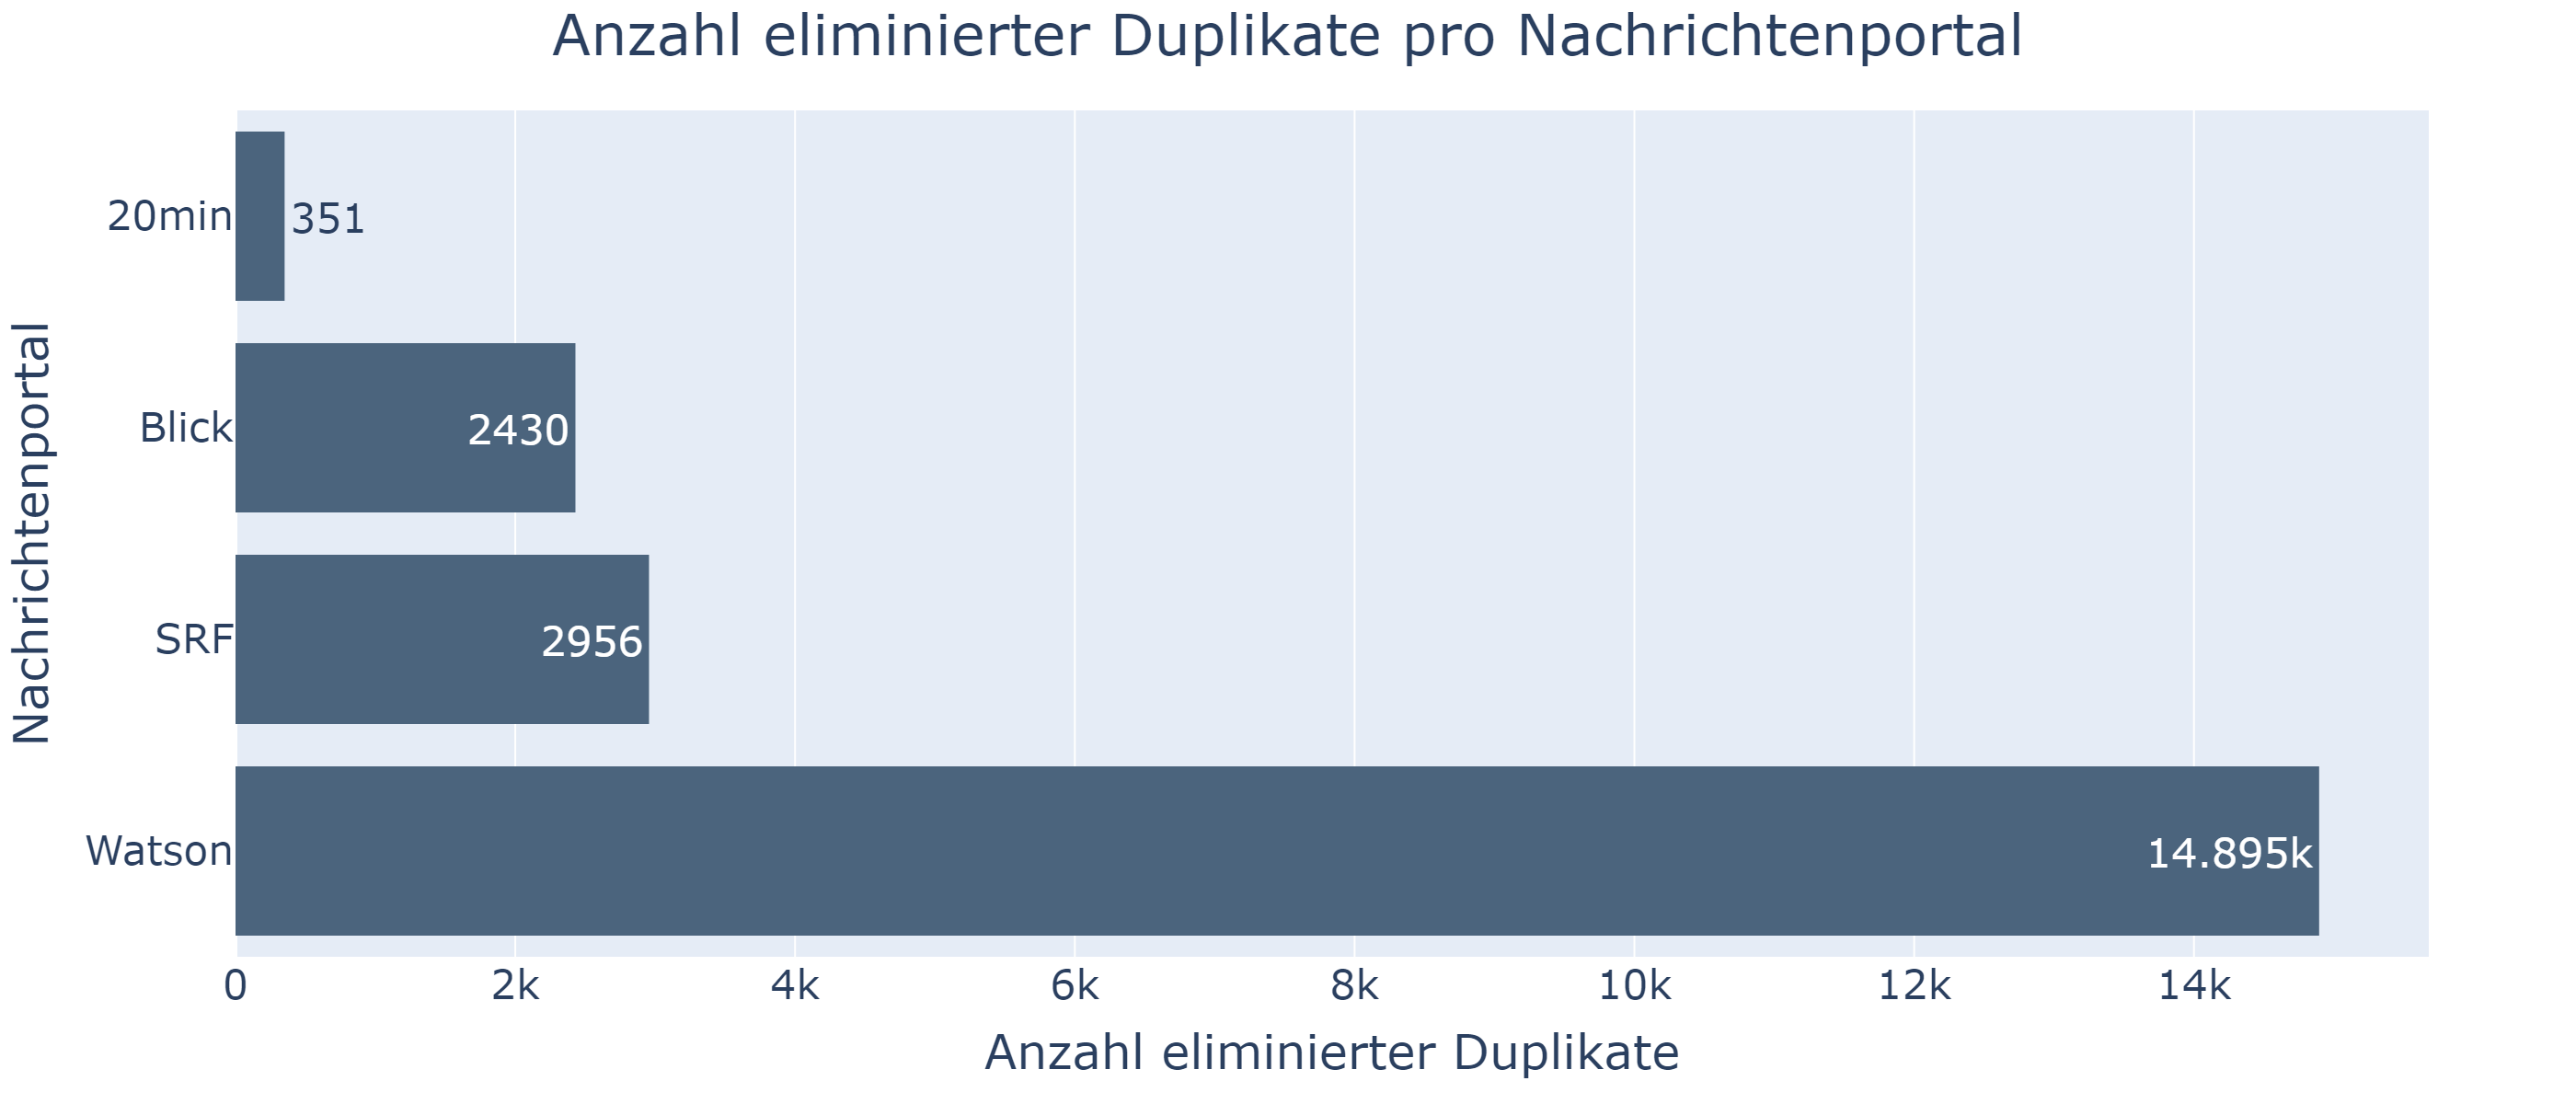
\includegraphics[width=1\linewidth]{./images/duplicates_count.png}
		\caption{Anzahl eliminierter Duplikate pro Nachrichtenportal}
		\label{duplicates}
	\end{center}
\end{figure}